\documentclass{ctexart}

\title{\Large 门电路测试与应用\\{\large 实验报告}}
\author{\large  信息科学技术学院 \quad 吴海\MyFont{垚} PB22051035 \\\large  信息科学技术学院 \quad 李\quad 毅 PB22051031 \\{教室:电四楼112室\quad 座位号:12}}
\date{2023年3月4日}
\usepackage{ctex}
\setCJKfamilyfont{myfont}{SimSun.ttf}
\newcommand{\MyFont}{\CJKfamily{myfont}}
\usepackage{amsmath}
\usepackage{amsfonts}
\usepackage{amssymb}
\usepackage{bm}
\usepackage{enumerate}
\usepackage{geometry}
\geometry{left=2.5cm,right=2.5cm,top=2cm,bottom=2cm}
\usepackage{fancyhdr}
\usepackage{lastpage}
\usepackage{booktabs}
\pagestyle{fancy}
\fancyhead[l]{ }
\fancyhead[r]{ }
\fancyhead[C]{
	\begin{tabular}{cclclc}
         & \multicolumn{4}{c}{\textbf{门电路测试与应用\quad 实验报告}}                                    &            \\
信息科学技术学院 & \multicolumn{2}{c}{PB22051035 吴海\MyFont{垚}} & \multicolumn{2}{c}{PB22051031 李毅} & 2024年3月4日
\end{tabular}
}
\fancyfoot[C]{ 第 {\thepage} 页,共 \pageref{LastPage} 页}
\renewcommand{\headrulewidth}{2pt}
\usepackage{graphicx}
\usepackage{geometry}
\usepackage[hidelinks]{hyperref}
\usepackage{multicol}
\usepackage{multirow}
\usepackage{ragged2e}
\usepackage[square,comma,numbers,super]{natbib}
\bibliographystyle{unsrt}
\usepackage{siunitx}
\usepackage{subfigure}
\usepackage{wrapfig}
\usepackage{xcolor}
\usepackage{cite}
\begin{document}
    \maketitle
    \thispagestyle{empty}
    
    \newpage 
    \setcounter{page}{1}

    \section*{第一部分 \quad 实验目的}
    \begin{enumerate}
        \item 熟悉数字逻辑电路实验箱的结构和用法
        \item 掌握数字逻辑电路测试方法与测试的原理
        \item 测试与门、或门、非门、与非门和异或门的逻辑功能
        \item 学习用基本逻辑门电路设计组合逻辑电路
    \end{enumerate}
    \section*{第二部分 \quad 实验原理}
    \subsection*{1.三种基本逻辑运算以及两种复合逻辑运算}

    \begin{minipage}[c]{0.6\textwidth}
        \centering
        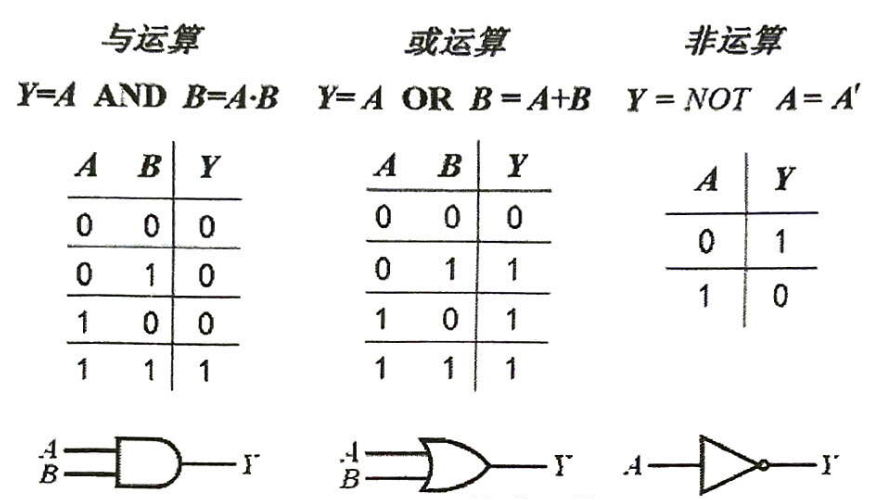
\includegraphics[width=1\linewidth]{2.1.png} 
        
    \end{minipage}
    \begin{minipage}[c]{0.4\textwidth}
        \centering
        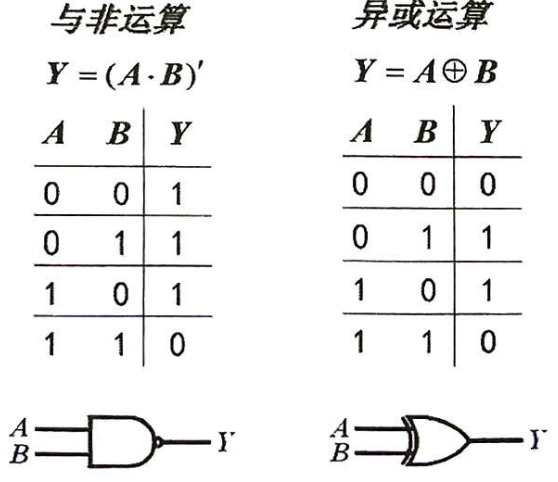
\includegraphics[width=1\linewidth]{2.2.png} 
        
    \end{minipage}
    \subsection*{2.组合逻辑电路设计方法}
    \begin{enumerate}[(1)]
        \item 抽象逻辑问题
        \item 写出逻辑真值表
        \item 写出逻辑表达式
        \item 画出卡诺图
        \item 简化逻辑表达式
        \item 画出逻辑电路图
    \end{enumerate}
    \subsection*{3.逻辑门电路功能与性能的测试}
    \begin{enumerate}[(1)]
        \item 静态测试法:给门电路输入端加固定的高低电平,用示波器,万用表或信号发光二极管(LED)测出门电路的输出响应。
        \item 动态测试法:给门电路输入端加一串脉冲信号,用示波器观测输入波形与输出波形的同步关系。
    \end{enumerate}
    \section*{第三部分 \quad 实验内容}
    \subsection*{1.验证各逻辑门的功能,列出真值表}
    \subsection*{1.1实验内容}
    以与非门74LS00为例,,输入端输入高低电平,输出端使用逻辑笔显示其逻辑功能,填写如下图表格并以同样方法测试74LS08 , 74LS32 , 74LS04 , 74LS86 , 74LS20
    \begin{figure}[htbp]
        \centering
        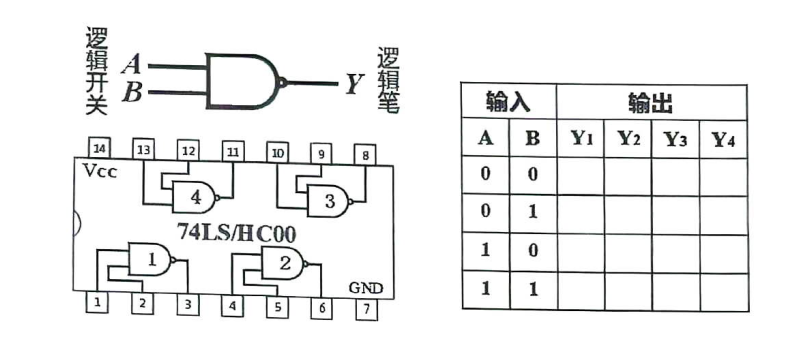
\includegraphics[width=17cm]{3.1.1.png}
    \end{figure}
    \subsection*{1.2实验数据}
    74LS00有(与非门):
     \begin{table}[!ht]
       \centering
       \caption{74LS00真值表}
       \begin{tabular}{|l|l|l|l|l|l|}
       \hline
        A & B & $Y_1$ & $Y_2$ & $Y_3$ & $Y_4$  \\ \hline
        0 & 0 & 1 & 1 & 1 & 1  \\ \hline
        0 & 1 & 1 & 1 & 1 & 1  \\ \hline
        1 & 0 & 1 & 1 & 1 & 1  \\ \hline
        1 & 1 & 0 & 0 & 0 & 0  \\ \hline
      \end{tabular}
    \end{table}

    74LS08有(与门):
    \begin{table}[!ht]
    \centering
    \caption{74LS08真值表}
    \begin{tabular}{|l|l|l|l|l|l|}
    \hline
        A & B & $Y_1$ & $Y_2$ & $Y_3$ & $Y_4$  \\ \hline
        0 & 0 & 0 & 0 & 0 & 0 \\ \hline
        0 & 1 & 0 & 0 & 0 & 0 \\ \hline
        1 & 0 & 0 & 0 & 0 & 0 \\ \hline
        1 & 1 & 1 & 1 & 1 & 1 \\ \hline
    \end{tabular}
    \end{table}
    
    74LS32有(或门):
    \begin{table}[!ht]
    \centering
    \caption{74LS32真值表}
    \begin{tabular}{|l|l|l|l|l|l|}
    \hline
        A & B & $Y_1$ & $Y_2$ & $Y_3$ & $Y_4$  \\ \hline
        0 & 0 & 0 & 0 & 0 & 0 \\ \hline
        0 & 1 & 1 & 0 & 0 & 0 \\ \hline
        1 & 0 & 1 & 0 & 0 & 0 \\ \hline
        1 & 1 & 1 & 1 & 1 & 1 \\ \hline
    \end{tabular}
    \end{table}
    
    74LS86(异或门):
    \begin{table}[!ht]
    \centering
    \caption{74LS86真值表}
    \begin{tabular}{|l|l|l|l|l|l|}
    \hline
        A & B & $Y_1$ & $Y_2$ & $Y_3$ & $Y_4$   \\ \hline
        0 & 0 & 0 & 0 & 0 & 0 \\ \hline
        0 & 1 & 1 & 0 & 0 & 0 \\ \hline
        1 & 0 & 1 & 0 & 0 & 0 \\ \hline
        1 & 1 & 0 & 0 & 0 & 0 \\ \hline
    \end{tabular}
    \end{table}
    
    对于该上四个电路,A分别对应1,4,9,12管脚,B分别对应2,5,10,13管脚,$Y_1 ,Y_2 , Y_3 , Y_4$分别对应3,6,8,11管脚

    74LS04有(非门):
    \begin{table}[!ht]
    \centering
    \caption{74LS04真值表}
    \begin{tabular}{|l|l|l|l|l|l|l|}
    \hline
        A & $Y_1$ & $Y_2$ & $Y_3$ & $Y_4$  & $Y_5$ & $Y_6$  \\ \hline
        0 & 1 & 1 & 1 & 1 & 1 & 1 \\ \hline
        1 & 0 & 0 & 0 & 0 & 0 & 0 \\ \hline
    \end{tabular}
    \end{table}

    对于上述电路,A对应1,3,5,9,11,13管脚,$Y_1 ,Y_2 , Y_3 , Y_4,Y_5 , Y_6$分别对应2,4,6,8,10,12管脚

    74LS20有(与非):
   \begin{table}[!ht]
    \centering
    \caption{74LS20真值表}
    \begin{tabular}{|c|c|c|c|c|c|c|c|c|c|c|c|c|c|c|c|c|}
    \hline
        A &  B & C & D & $Y_1$ & $Y_2$ & A &  B & C & D & $Y_1$ & $Y_2$ \\ \hline
        0 & 0 & 0 & 0 & 1 & 1 & 1 & 0 & 0 & 0 & 1 & 1 \\ \hline
        0 & 0 & 0 & 1 & 1 & 1 & 1 & 0 & 0 & 1 & 1 & 1 \\ \hline
        0 & 0 & 1 & 0 & 1 & 1 & 1 & 0 & 1 & 0 & 1 & 1 \\ \hline
        0 & 0 & 1 & 1 & 1 & 1 & 1 & 0 & 1 & 1 & 1 & 1 \\ \hline
        0 & 1 & 0 & 0 & 1 & 1 & 1 & 1 & 0 & 0 & 1 & 1 \\ \hline
        0 & 1 & 0 & 1 & 1 & 1 & 1 & 1 & 0 & 1 & 1 & 1 \\ \hline
        0 & 1 & 1 & 0 & 1 & 1 & 1 & 1 & 1 & 0 & 1 & 1 \\ \hline
        0 & 1 & 1 & 1 & 1 & 1 & 1 & 1 & 1 & 1 & 0 & 0 \\ \hline
    \end{tabular}
\end{table}

    由上述数据总结可得,各逻辑门真值表都符合对应逻辑门的逻辑关系,逻辑门功能正常。
    \subsection*{2.动态测试}
    \subsection*{2.1实验内容}
    选用一个与非门按下图连线,将一个输入端接连续脉冲源(频率为20KHZ),S接任意逻辑电平开关,用示波器观察并记录S分别为高电平H和低电平L时的输出波形。并推广到与门,或门,异或门。
    \begin{figure}[htbp]
        \centering
        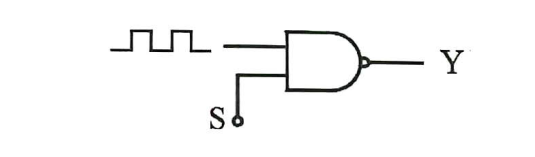
\includegraphics[width=13cm]{3.2.1.png}
    \end{figure}
    \subsection*{2.2实验数据}
    实验所得数据如下:
    
    \begin{minipage}[c]{0.6\textwidth}
        \centering
        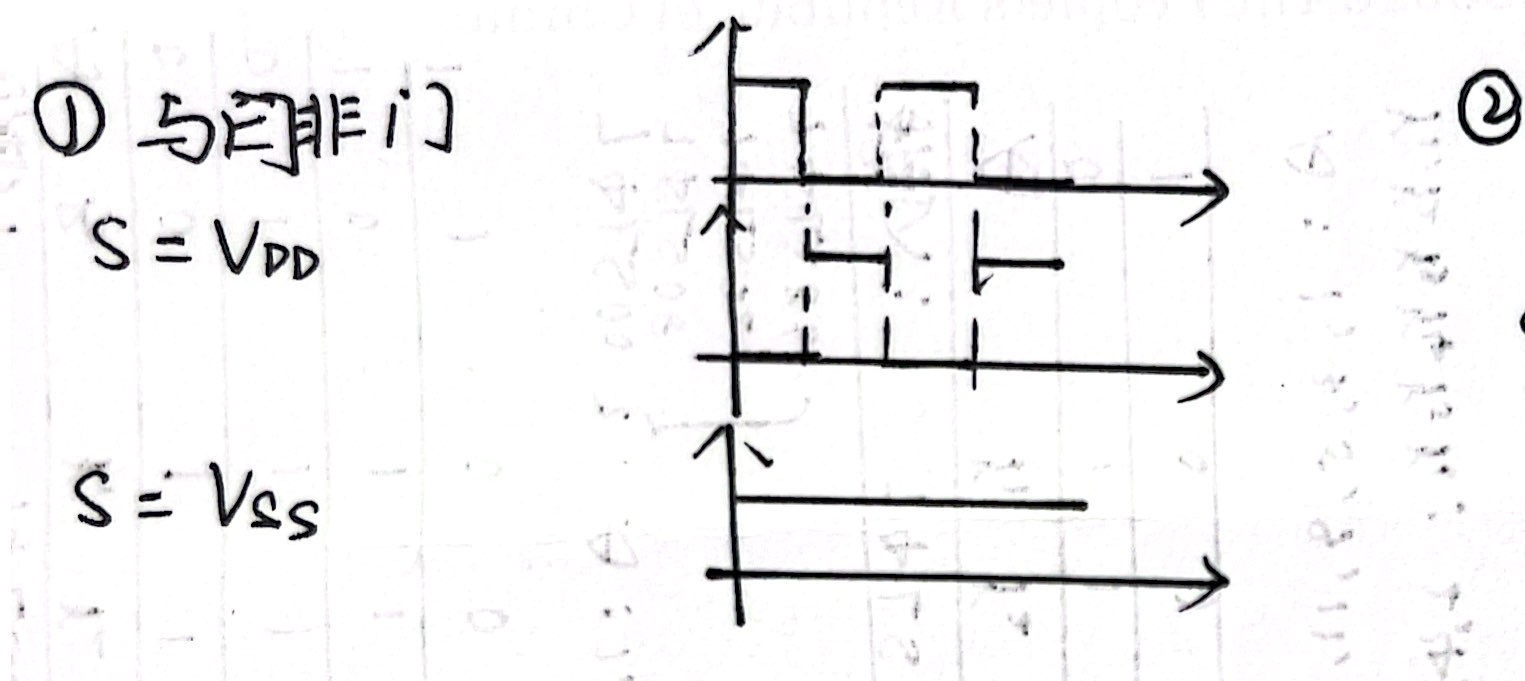
\includegraphics[width=1\linewidth]{3.2.1.JPG} 
    \end{minipage}
    \begin{minipage}[c]{0.4\textwidth}
        \centering
        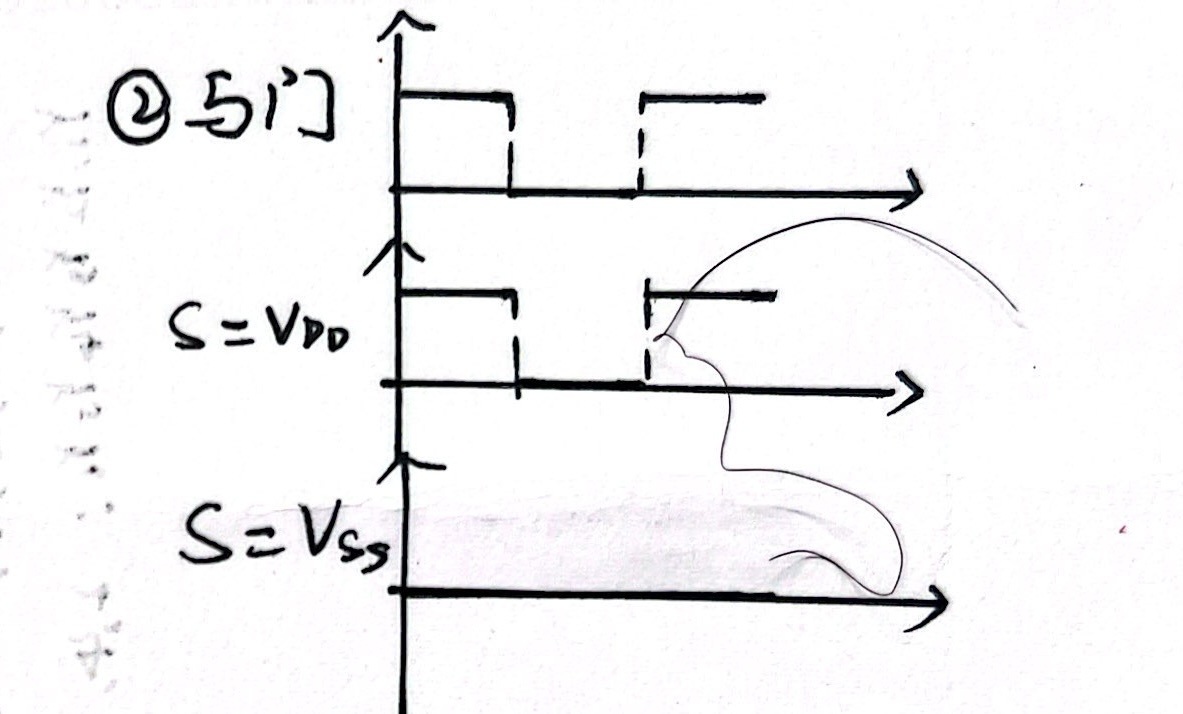
\includegraphics[width=1\linewidth]{3.2.2.JPG} 
    \end{minipage}
    \begin{minipage}[c]{0.6\textwidth}
        \centering
        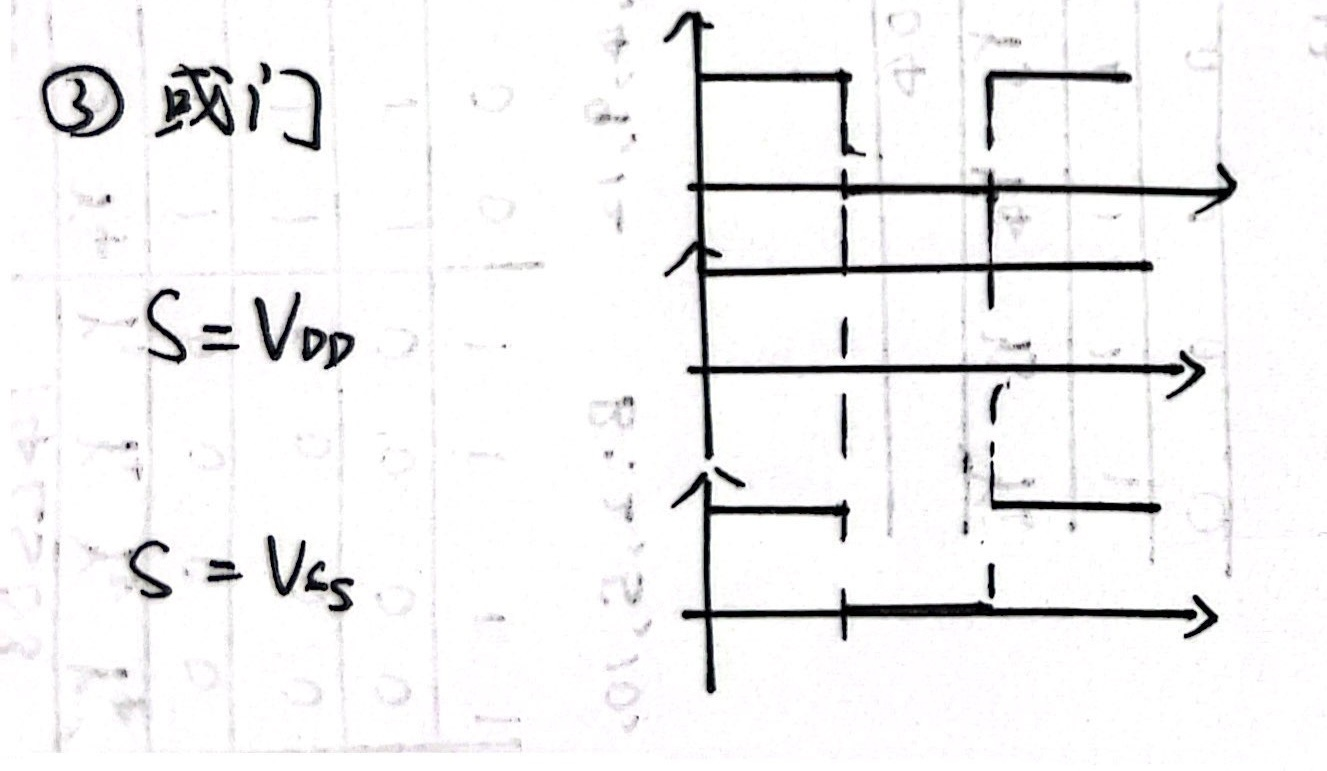
\includegraphics[width=1\linewidth]{3.2.3.JPG} 
    \end{minipage}
    \begin{minipage}[c]{0.4\textwidth}
        \centering
        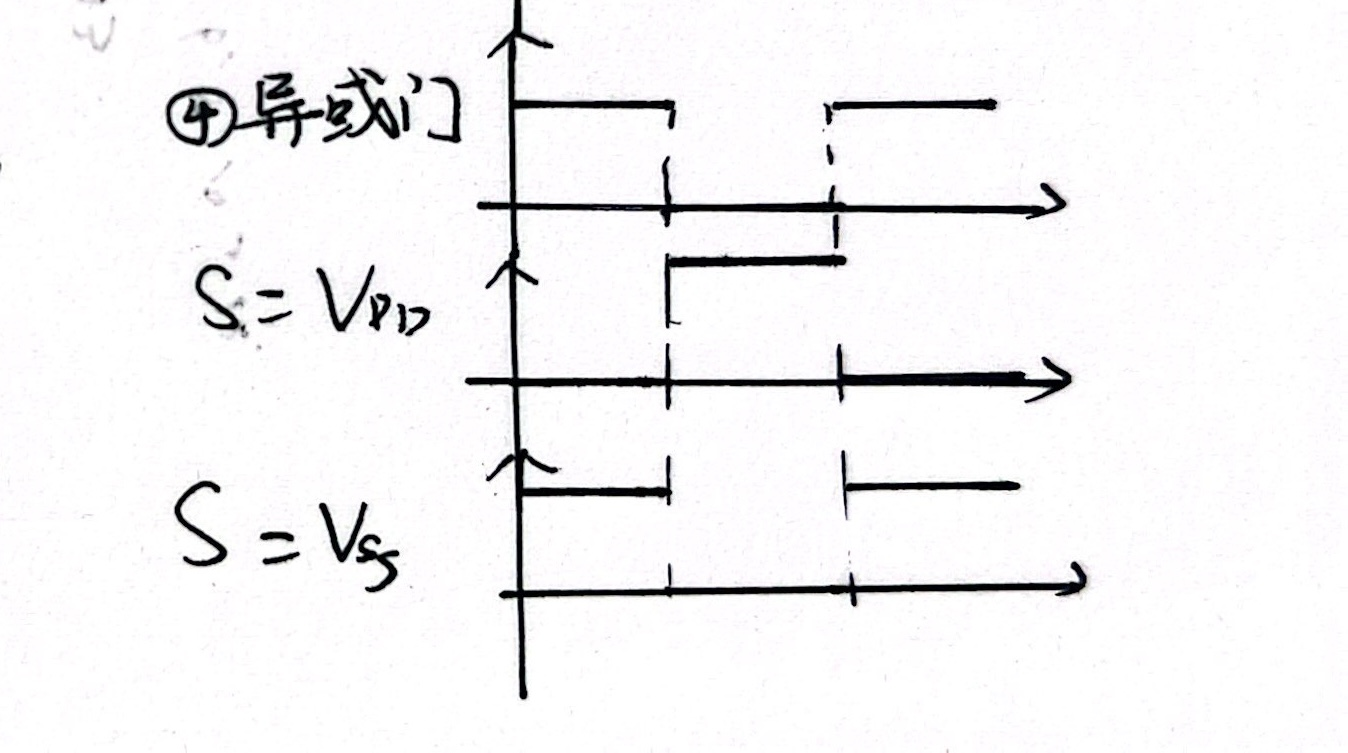
\includegraphics[width=1\linewidth]{3.2.4.JPG} 
    \end{minipage}
    
    \subsection*{3.设计开关电路}
    \subsection*{3.1实验内容}
    设计一个用A,B,C,D四个开关控制一盏灯L的电路,要求改变任何一个开关状态都能使L的状态发生改变
    \subsection*{3.2实验设计}
    根据题意四个开关改变任何一个都能使电路状体发生改变,因为常规逻辑都不能保证任改变一个输入都会使得输出发生改变,因此想到特殊逻辑门异或门,对于异或门任意一个输入改变都会改变结果,因此考虑将四个输入以异或门连接。
    \begin{equation}
        Y=A\oplus B\oplus C\oplus D\notag
    \end{equation}
    逻辑电路图如下:
    \begin{figure}[htbp]
        \centering
        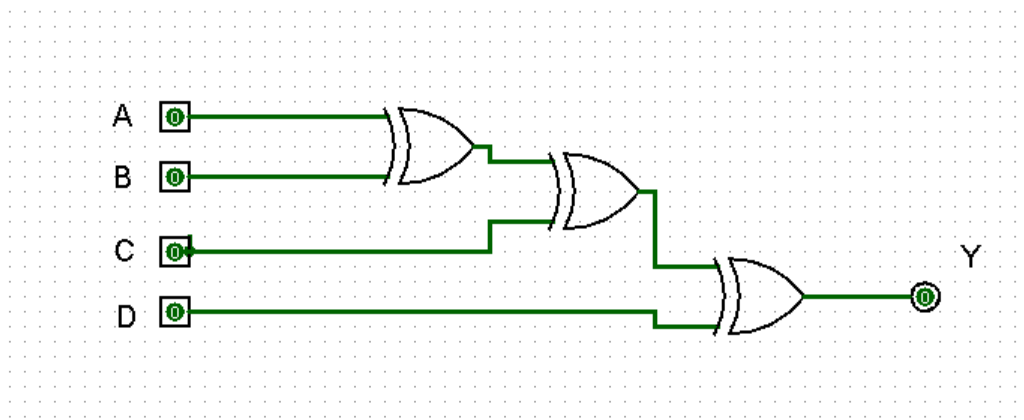
\includegraphics[width=15cm]{3.3.1.png}
    \end{figure}
    \subsection*{4.设计数字锁}
    \subsection*{4.1实验内容}
    设计一个保险箱用的思维代数数字锁,4位代码A,B,C,D四个输入端和一个开锁用的钥匙孔输入端E,当开锁时(E=1)如果输入的代码与设定的密码相同,则保险箱打开(Y=1),否则电路发出警报信号(Z=1)
    \subsection*{4.2实验设计}
    本此设计初始密码为1111,因为本题逻辑关系过于简单,因此可直接写出Y,Z的逻辑表达式为:
    \begin{equation}
        Y=EABCD=(E'+(ABCD)')'\notag 
    \end{equation}
    \begin{equation}
        Z=E'+E(ABCD)'\notag
    \end{equation}
    对于Y的逻辑表达式,因为本次实验没有五个变量的与门,因此变换成与非形式,至于没有的或非门可以用或门与非门实现。

    所得逻辑电路图如下:
    \begin{figure}[htbp]
        \centering
        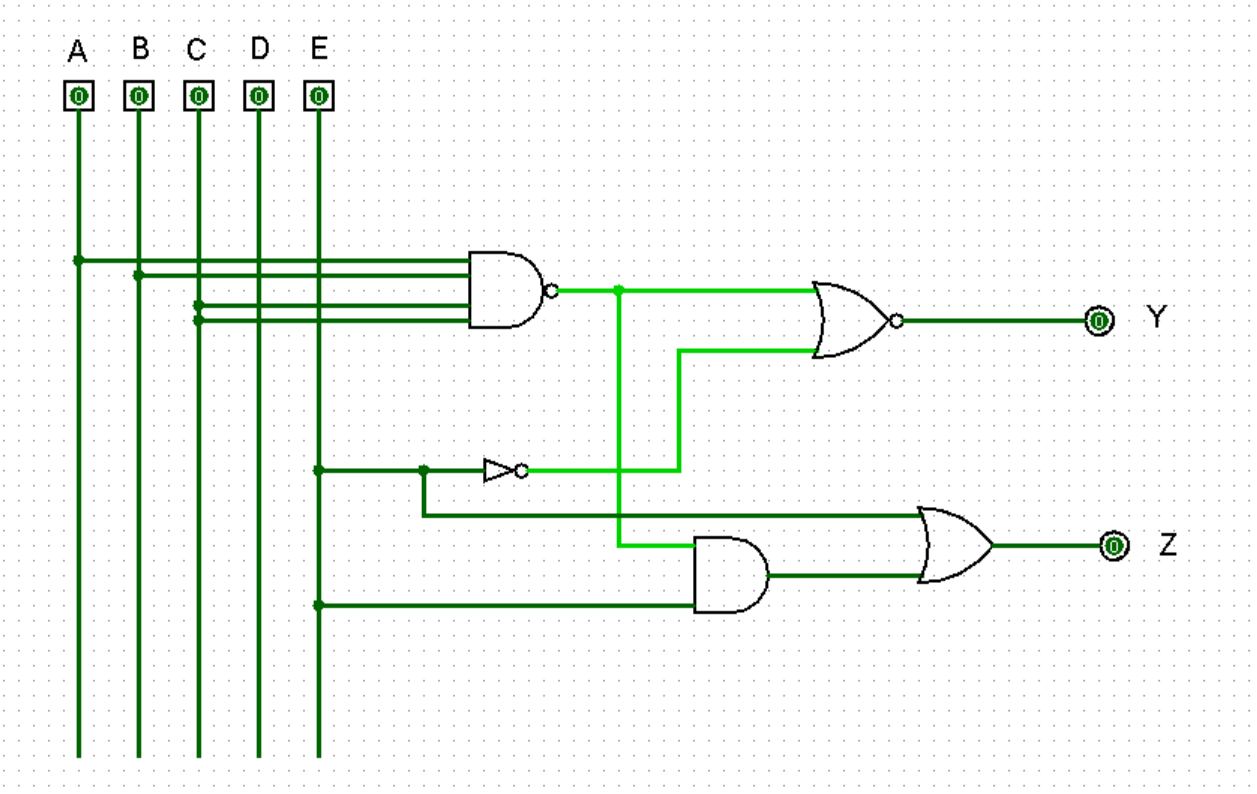
\includegraphics[width=16cm]{3.4.1.png}
    \end{figure}

    \newpage
    \subsection*{5.设计全加器}
    \subsection*{5.1实验内容}
    设计一个全加器,要求使用异或门和与非门
    \subsection*{5.2设计电路}
    根据题意列出真值表为:
    \begin{table}[!ht]
    \centering
    \caption{全加器真值表}
    \begin{tabular}{|c|c|c|c|c|}
    \hline
        A & B &  CI & Y & CO \\ \hline
        0 & 0 & 0 & 0 & 0 \\ \hline
        0 & 1 & 0 & 1 & 0 \\ \hline
        1 & 0 & 0 & 1 & 0 \\ \hline
        1 & 1 & 0 & 0 & 1 \\ \hline
        0 & 0 & 1 & 0 & 0 \\ \hline
        0 & 1 & 1 & 1 & 1 \\ \hline
        1 & 0 & 1 & 1 & 1 \\ \hline
        1 & 1 & 1 & 0 & 1 \\ \hline
    \end{tabular}
    \end{table}

    其中CI为进位输入,CO为进位输出,Y为该位输出。

    因此有:
    \begin{align*}
        Y &=A'B CI'+AB'CI'+A'B'CI+AB CI\\
          &=CI'(A\oplus B)+CI(A\oplus B)'\\
          &=[CI \oplus (A\oplus B)]
    \end{align*}
    \begin{align*}
        CO &=AB CI'+ABCI+A'BCI+AB'CI+A'B CI\\
          &=CI'(A\oplus B)+CI(A\oplus B)'\\
          &={[A(CI\oplus B)]'(BC)'}'
    \end{align*}
    
    \subsection*{6.水位监测元件}
    \subsection*{6.1实验内容}
    用X,Y两个水泵给水箱供水,水箱内从高到低有A,B,C三个水位检测元件,要求水位在C点一下,X,Y同时工作;水位在B,C之间,X工作;在A,B之间,Y工作;高于A点,两台水泵停止工作
    \subsection*{6.2设计电路}
    首先对实验进行抽象,令水位高于水位监测元件时该元件为1,水位低于时元件为0.同时注意由于现实的物理特性,A,B,C分别按照从高到低分布,因此如ABC对应100,110,101,010在物理上不可能出现,因此为无关项,画卡诺图化简时可以使用。

    实验所得真值表为;
    \begin{table}[!ht]
    \centering
    \caption{水箱问题真值表}
    \begin{tabular}{|c|c|c|c|c|}
    \hline
        A & B & C & X & Y \\ \hline
        0 & 0 & 0 & 1 & 1 \\ \hline
        0 & 0 & 1 & 1 & 0 \\ \hline
        0 & 1 & 1 & 0 & 1 \\ \hline
        1 & 1 & 1 & 0 & 0 \\ \hline
    \end{tabular}
    \end{table}

    利用卡诺图及其无关项化简可得:
    \begin{equation*}
        X=B'
    \end{equation*}
    \begin{equation*}
        Y=C'+A'B
    \end{equation*}
    \newpage
    \section*{第四部分 \quad 思考题}
    \subsection*{1.为了判断74LS20逻辑功能是否正常,至少要测量几组输入?}
    要全面测试74LS20的逻辑功能,需要覆盖所有可能的输入组合,以确保其在各种情况下都能正确执行逻辑功能。74LS20由两个四输入与非门组成,故至少需要测量$2\times2^4=32$组输入。

    \subsection*{2.用与非门和异或门设计一可逆的4位码制变换器}
    设计要求:

    (1)在控制信号C=1,它将8421码转换为格雷码;C=0时,它将格雷码转换8421码;

    (2)写出设计步骤,列出码变换真值表并画出逻辑电路图。

    列出真值表如表4.1所示:
    \begin{table}[!ht]
\centering 表4.1 可逆4位码制变换器真值表
\begin{tabular}{|cccc|c|cccc||cccc|c|cccc|}
\hline
$A_1$ & $A_2$ & $A_3$ & $A_4$ & C & $B_1$ & $B_2$ & $B_3$ & $B_4$ & $A_1$ & $A_2$ & $A_3$ & $A_4$ & C & $B_1$ & $B_2$ & $B_3$ & $B_4$ \\ \hline
0     & 0     & 0     & 0     & 1 & 0     & 0     & 0     & 0     & 0     & 0     & 0     & 0     & 0 & 0     & 0     & 0     & 0     \\ \hline
0     & 0     & 0     & 1     & 1 & 0     & 0     & 0     & 1     & 0     & 0     & 0     & 1     & 0 & 0     & 0     & 0     & 1     \\ \hline
0     & 0     & 1     & 0     & 1 & 0     & 0     & 1     & 1     & 0     & 0     & 1     & 1     & 0 & 0     & 0     & 1     & 0     \\ \hline
0     & 0     & 1     & 1     & 1 & 0     & 0     & 1     & 0     & 0     & 0     & 1     & 0     & 0 & 0     & 0     & 1     & 1     \\ \hline
0     & 1     & 0     & 0     & 1 & 0     & 1     & 1     & 0     & 0     & 1     & 1     & 0     & 0 & 0     & 1     & 0     & 0     \\ \hline
0     & 1     & 0     & 1     & 1 & 0     & 1     & 1     & 1     & 0     & 1     & 1     & 1     & 0 & 0     & 1     & 0     & 1     \\ \hline
0     & 1     & 1     & 0     & 1 & 0     & 1     & 0     & 1     & 0     & 1     & 0     & 1     & 0 & 0     & 1     & 1     & 0     \\ \hline
0     & 1     & 1     & 1     & 1 & 0     & 1     & 0     & 0     & 0     & 1     & 0     & 0     & 0 & 0     & 1     & 1     & 1     \\ \hline
1     & 0     & 0     & 0     & 1 & 1     & 1     & 0     & 0     & 1     & 1     & 0     & 0     & 0 & 1     & 0     & 0     & 0     \\ \hline
1     & 0     & 0     & 1     & 1 & 1     & 1     & 0     & 1     & 1     & 1     & 0     & 1     & 0 & 1     & 0     & 0     & 1     \\ \hline
1     & 0     & 1     & 0     & 1 & 1     & 1     & 1     & 1     & 1     & 1     & 1     & 1     & 0 & 1     & 0     & 1     & 0     \\ \hline
1     & 0     & 1     & 1     & 1 & 1     & 1     & 1     & 0     & 1     & 1     & 1     & 0     & 0 & 1     & 0     & 1     & 1     \\ \hline
1     & 1     & 0     & 0     & 1 & 1     & 0     & 1     & 0     & 1     & 0     & 1     & 0     & 0 & 1     & 1     & 0     & 0     \\ \hline
1     & 1     & 0     & 1     & 1 & 1     & 0     & 1     & 1     & 1     & 0     & 1     & 1     & 0 & 1     & 1     & 0     & 1     \\ \hline
1     & 1     & 1     & 0     & 1 & 1     & 0     & 0     & 1     & 1     & 0     & 0     & 1     & 0 & 1     & 1     & 1     & 0     \\ \hline
1     & 1     & 1     & 1     & 1 & 1     & 0     & 0     & 0     & 1     & 0     & 0     & 0     & 0 & 1     & 1     & 1     & 1     \\ \hline
\end{tabular}
\end{table}

写出逻辑表达式并使用公式法化简:
\begin{align*}
    B_1=A_1  
\end{align*}
\begin{align*}
   B_2&=C(A_1\oplus A_2)+C'(A_1 \oplus A_2) \\
        &=A_1\oplus A_2 \\ 
\end{align*}
\begin{align*}
    B_3&=C(A_2\oplus A_3)+C'(A_1\oplus A_2 \oplus A_3) \\
    &=C(A_2\oplus A_3)+C'A_1(A_2 \oplus A_3)'+C'A'_1(A_2 \oplus A_3) \\
    &=(C'A_1)'(A_2\oplus A_3)+C'A_1(A_2 \oplus A_3)' \\
    &=(C'A_1)\oplus(A_2\oplus A_3) \\
\end{align*}
\begin{align*}
    B_4&=C(A_3\oplus A_4)+C'(A_1\oplus A_2 \oplus A_3 \oplus A_4) \\
    &=C(A_3\oplus A_4)+C'(A_1\oplus A_2)(A_3 \oplus A_4)'+C'(A_1\oplus A_2)'(A_3 \oplus A_4) \\
    &=(C'(A_1\oplus A_2))'(A_3 \oplus A_4)+C'(A_1\oplus A_2)(A_3 \oplus A_4)' \\
    &=C'(A_1\oplus A_2)\oplus(A_3 \oplus A_4)
\end{align*}

用与非门和异或门搭出逻辑电路图如下:

    \begin{minipage}[c]{\textwidth}
        \centering 
        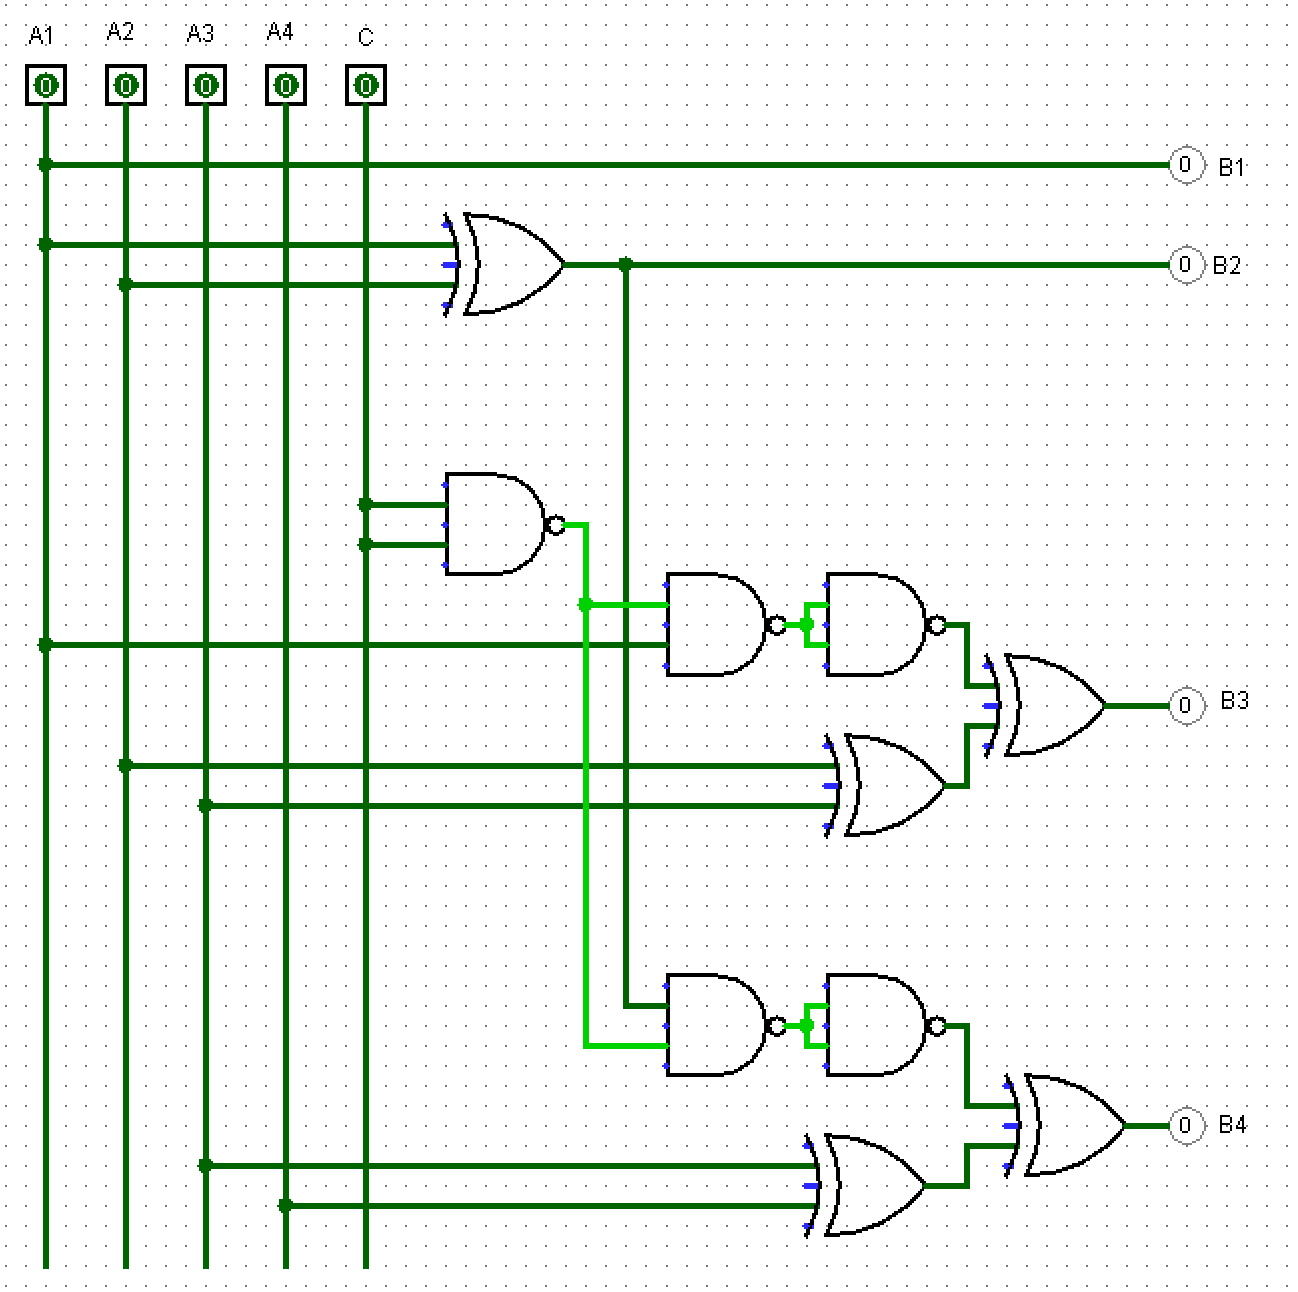
\includegraphics[width=0.9\linewidth]{4.png} 
        
        图4:可逆4位码制变换器逻辑电路图
    \end{minipage}


\end{document}

